\documentclass[paper=a4]{scrartcl}	
\newcommand{\mvec}[1]{\ensuremath{\mathbf{#1}}} 
\newcommand{\mvect}[2]{\ensuremath{\mathbf{#1}_\mathrm{#2}}} 
\newcommand{\Heff}{\ensuremath{\mvec{H}_\mathrm{eff}}} 
\newcommand{\uv}[1]{\ensuremath{\mathbf{\hat{#1}}}} % for unit vector
\newcommand{\abs}[1]{\left| #1 \right|} % for absolute value
\newcommand{\avg}[1]{\left< #1 \right>} % for average

\usepackage[english]{babel}															% English language/hyphenation
\usepackage[protrusion=true,expansion=true]{microtype}				% Better typography
\usepackage{amsmath,amsfonts,amsthm}										% Math packages
\usepackage[pdftex]{graphicx}														% Enable pdflatex
\usepackage{url}
\usepackage{amsmath,amssymb}
\usepackage{epsfig}
\usepackage{subfig}
\usepackage{verbatim}
\usepackage{listings}
\usepackage{color}
\usepackage{textcomp}
\usepackage{multirow}
\usepackage[thinlines]{easytable}
\definecolor{listinggray}{gray}{0.9}
\definecolor{lbcolor}{rgb}{0.9,0.9,0.9}
\lstset{
	backgroundcolor=\color{lbcolor},
	tabsize=4,
	rulecolor=,
	language=python,
        basicstyle=\scriptsize,
        upquote=true,
        aboveskip={1.5\baselineskip},
        columns=fixed,
        showstringspaces=false,
        extendedchars=true,
        breaklines=true,
        prebreak = \raisebox{0ex}[0ex][0ex]{\ensuremath{\hookleftarrow}},
        frame=single,
        showtabs=false,
        showspaces=false,
        showstringspaces=false,
        identifierstyle=\ttfamily,
        keywordstyle=\color[rgb]{0,0,1},
        commentstyle=\color[rgb]{0.133,0.545,0.133},
        stringstyle=\color[rgb]{0.627,0.126,0.941},
}


\usepackage{sectsty}												
%\allsectionsfont{\normalfont\scshape}
%\allsectionsfont{\centering \normalfont\scshape}

\begin{document}

\title{ \Large Demag with macrogeometry (PBC)}
\author{\normalsize Weiwei Wang}
\date{\normalsize \today}
\maketitle

\section{Original problem}

For the given magnetic sample, the demag field can be computed as gradient of a magnetic scalar potential $\phi$,
\begin{equation}\label{eq_h}
\mvect{H}{d} = - \nabla \phi
\end{equation}
The magnetic potential satisfies the equation
\begin{equation}\label{eq_h}
\nabla^2 \phi = - \rho_m
\end{equation}
where $\rho_m = - \nabla \cdot \mvec{M}$. Therefore, outside of the sample $ \rho_m =0$. At the boundary we have,
\begin{align}
\phi^{+} &= \phi^{-} \\
(\nabla \phi^{-} - \nabla \phi^{+}) \cdot \mvec{n} &= \sigma_m
\end{align}
where $\sigma_m = \mvec{M} \cdot \mvec{n}$ and the potential is assumed to be zero at infinity.

\section{FK's approach}
Split the potential into two parts, $\phi = \phi_1+\phi_2$, where $\phi_1$ is assumed to solve a closed boundary problem,
and $\phi_2$ should hold the total potential in the original problem.
The $\phi_1$ is chosen to be 
\begin{align}
\nabla^2 \phi_1 =  \nabla \cdot \mvec{M} \;\;\; \text{for } \mvec{r} \in V\\
\nabla^2 \phi_1 = 0 \;\;\; \text{for } \mvec{r} \not\in V
\end{align}
and the natural boundary conditions hold for $\phi_1$, 
\begin{equation}\label{eq_h}
\nabla \phi_1 \cdot \mvec{n} = \mvec{M} \cdot \mvec{n} \;\;\; \text{for } \mvec{r} \in \partial V\\
\end{equation}
Therefore $\phi_2$ needs to satisfy the Laplace equation everywhere in space, 
\begin{align}
\nabla^2 \phi_2 &=  0\\
(\nabla \phi_2^{-} - \nabla \phi_2^{+}) \cdot \mvec{n} &= 0\\
\phi_2^{-} - \phi_2^{+} &= \phi_1^{-} 
\end{align}
It turns out $\phi_2$ has the following solution, 
\begin{equation}\label{eq_U2}
\phi_2(\mvec{r})=\frac{1}{4\pi}\oint_{\partial V} \phi_1 (\mvec{x}) \nabla_x \frac{1}{|\mvec{r}-\mvec{x}|}\cdot \mvec{n}_x \mathrm{d}S
+\left( \frac{\Omega(\mvec{r})}{4\pi}-1 \right) \phi_1(\mvec{r}).
\end{equation}
where we have taken the limit $\mvec{r} \rightarrow \partial V$ from the inner of the sample (am I correct here?). 
By inserting the basis functions into equation (\ref{eq_U2}) one arrives at 
\begin{equation}
\Phi_2 = \mvec{B} \Phi_1
\end{equation}
where $\mvec{B}$ is a dense matrix. In practice, $B$ can be computed by Lindholm-formula.

\section{Implementation of FK}
In our code, to compute the demag field we need the following steps,
\begin{enumerate}
  \item compute $\phi_1$ in the sample
  \item extract $\phi_1$ at the boundary
  \item build the matrix $\mvec{B}$
  \item compute the $\phi_2$ at the boundary
  \item solve $\phi_2$ in the sample by using the known $\phi_2$ at the boundary
  \item sum $\phi_1$ and $\phi_2$ to obtain $\phi$ 
  \item compute the demag field from $\phi$
\end{enumerate}

\section{Macrogeometry (PBC)}
What we need to implement the Macrogeometry (PBC) is to change the dense matrix $B$, and we keep other
steps exactly the same as FK method. Here we have a tiny improvement in building the dense matrix $B$:
we have removed the small gap in our code. Our solution is based on the assumption that in the limit 
case the Lindholm-formula gives the solid angle of the triangle and approaching path. Clearly, this 
solid angle depends on the approaching path, which is not unique. However, in our case we can consider the 
approaching path as the given translation vector.

\section{Tests}
\subsection{Demag field}
We consider a cube with dimensions $10\times 10 \times 10$ nm$^3$ and apply the macrogeometry condition in $x$ direction. 
The effective field as a function of the number of the copies are shown in the following figure, 
\begin{figure}[tbhp]
\begin{center}
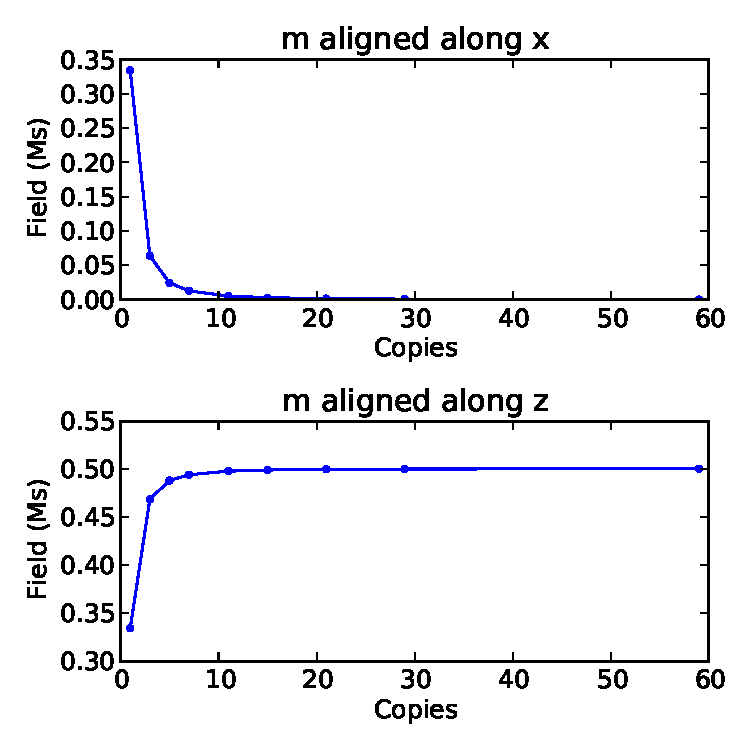
\includegraphics[scale=0.8]{figure/fields.pdf} 
\caption{The demag field as a function of the number of the copies.}
\label{fig_demag}
\end{center}
\end{figure}

\subsection{Frequency}
The sample is the same as the last example, and we choose $n=49$ copies of the sample in $x$ direction. 
\begin{figure}[tbhp]
\begin{center}
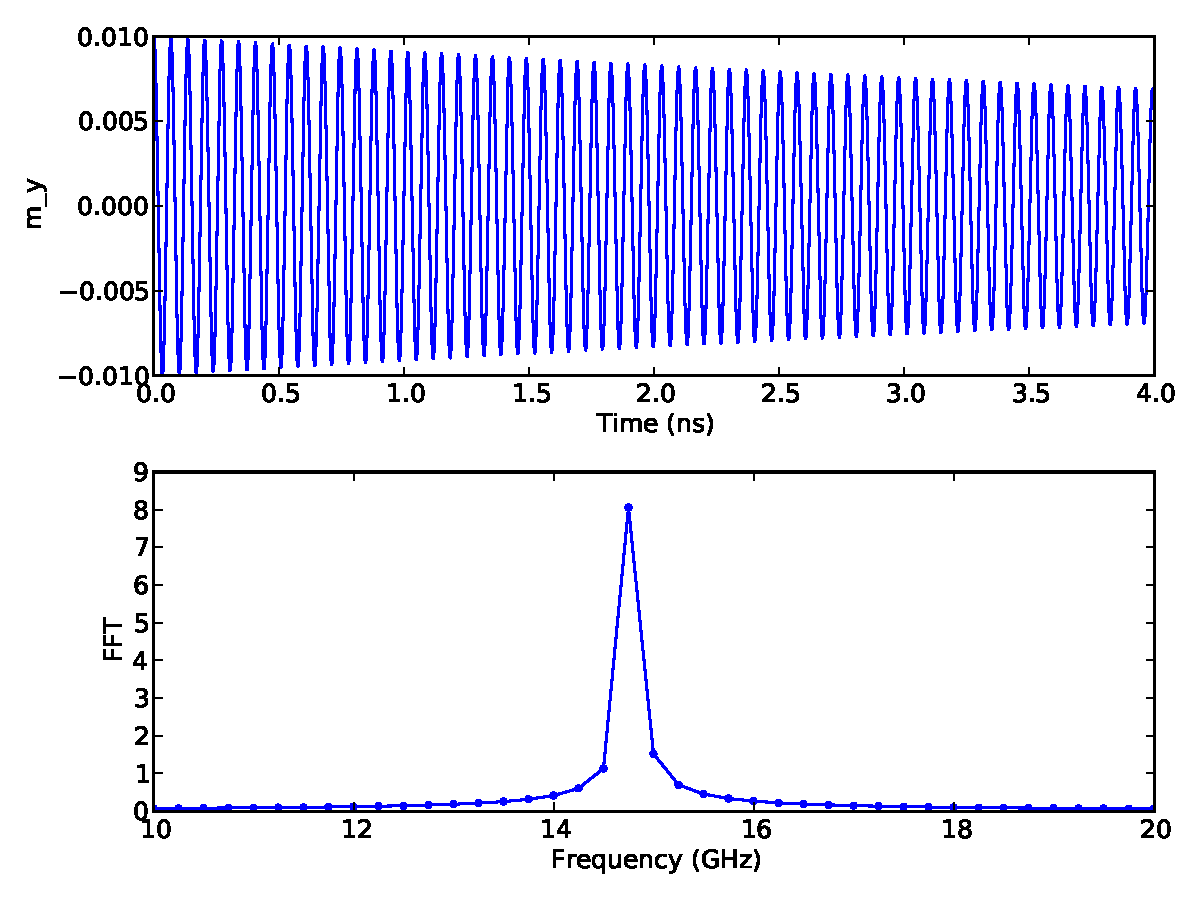
\includegraphics[scale=0.46]{figure/average_fft.pdf} 
\caption{The frequency obtained using ring-down method.}
\label{fig_freq}
\end{center}
\end{figure}
Figure \ref{fig_freq} shows the FFT spectrum of the $m_y$ component of the magnetisation,  we can find that the 
resonance frequency is close to $15$ GHz.
The expected resonance frequency for a infinity long rod is $\omega = 1/2 \gamma M_s$, i.e., $f=\omega/(2 \pi) = 15.1$ GHz. Therefore, it seems 
we can get the correct result using macrogeometry. 


%\bibliographystyle{unsrt}
%\bibliography{srk,sllg}

\end{document}
